Overview (0.5 page) (AJ, JP)
\begin{itemize}
  \item "Technical Part" (AJ)
  \item SES
  \item Cavity
  \item Ray-casting + parameters for vis
\end{itemize}

\subsection{Overview}

Overview of the algorithm: (JP)
\begin{itemize}
  \item Per frame we perform the following steps: ...
  \item The data comes in form of trajectories describing motion of individual atoms, we do not assume anything about the data.
  \item We split computations to two groups, which are performed on per frame basis.
	\begin{enumerate}
	  \item Data preprocessing (surface, cavity and attributes computations)
		\item Visualization  (ray-casting, opacity calculation, etc.)
	\end{enumerate}
\end{itemize}

\begin{figure*}[htb]
  \centering
  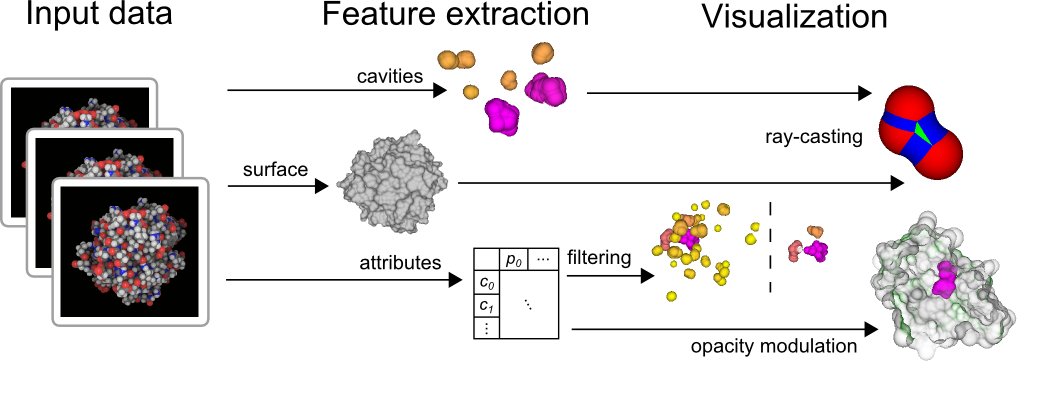
\includegraphics[width=7.3in]{image/overview.png}
  \caption{\textcolor{red}{TODO}.}
	\label{fig:overview}
\end{figure*}

\subsection{Extended CB Algorithm}

Our extended CB algorithm is based on the existing research that utilizes the GPU capabilities~\cite{krone2011parallel}.
In the former study, the SES is represented as three different sets of surface primitives -- spheres, tori, and spherical triangles, that are ray-casted to obtain opaque surface visualization. 
While ray-casting spheres and tori, some sections of the final image will be later occluded by the spherical triangles.
\textcolor{red}{JP: This needs to be explained: Therefore, to visualize contour surface representation using transparency}, we extended the algorithm so that it computes a SES represented with:
\begin{itemize}
	\item Spherical triangles.
  \item Toroidal patches -- a toroidal patch is delimited by two spherical triangles.
	\item Spherical patches -- a spherical patch is enclosed by edges of three or more toroidal patches.
\end{itemize}

\textcolor{red}{TODO Check if it's correct: In comparison with the previous solution our main contribution here lies in the computation of toroidal and spherical patches.
Using them we avoid the situation when the previous algorithm renders parts of tori and spheres which do not form the final surface.}

Kauker et al.~\cite{kauker2013rendering} proposed to ray-cast a toroidal patch using a torus and two clipping planes defined by its delimiting triangles.
<<<<<<< Updated upstream
We modify the data structure used to store spherical triangles in such a way that all spherical triangles that delimit patches on a torus are known. Therefore, it allows us to ray-cast toroidal patches instead of tori.
In order to get all triangles incident to some torus, we hash the triangles by three keys -- one for each torus which is connected to a triangle.
We implemented a simple hash table which is based on linear addressing scheme with quadratic probing \cite{alcantara2011efficient}.
=======
We modify the data structure used to store spherical triangles in such a way that all spherical triangles that delimit patches on a torus are known. Therefore, it allows us to ray-cast toroidal patches directly instead of tori.
In order to get all triangles incident to some torus, we hash the triangles by three keys --- one for each torus which is connected to a triangle.
We implemented a simple hash table which is based on linear addressing scheme with quadratic probing.
For more details regarding the hashing technique see \cite{alcantara2011efficient}.
>>>>>>> Stashed changes

Since a spherical patch is bounded by toroidal patches, we extended the original algorithm by adding three new GPU kernels that compute the sets of toroidal patches forming the spherical patches (see Section~\ref{sec:graph}).
When visualizing the surface, each such set is used to ray-cast a spherical patch (see Section~\ref{sec:spherical-patches}).

\begin{figure}[htb]
  \centering
  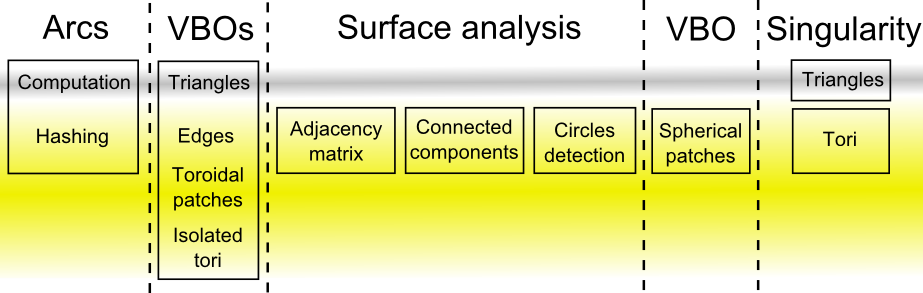
\includegraphics[width=3.3in]{image/kernels.png}
  \caption{Overview of our extended algorithm.
	The algorithm steps are ordered from the left to the right.
	GPU kernels are marked with squares containing both original (grey) and our novel parts (yellow).}
	\label{fig:kernels}
\end{figure}

\subsection{Surface graph}
\label{sec:graph}
   
%\begin{itemize}
%  \item Idea: computed surfaces are continuous (closed) and graphs of their primitives form isolated components in the whole graph of all surface primitives
%  \item Modification of parallel CB of Krone et. al --- aaaa
%  \item Extension of parallel CB of Krone et. al --- 3 new kernels:
%	\begin{enumerate}
%	  \item Adjacency matrix is built (only 3 edges at each vertex)
%    \item Labeling of connected components (parallel BFS --- suboptimal)
%    \item Circles of edges for each spherical patch are computed
%  \end{enumerate}
%  \item Assign spheres with edges
%  \item Detect circles in edges --- bubble sort $O(n^2)$
%  \item Step 3 --- one sphere can form two or more surfaces
%  \item Rendering of spherical patches --- spherical polygons
%  \item Odd-even rule + point outside polygon
%  \item Special case: isolated tori
%\end{itemize}

The computed surface contains primitives of both the outer molecular surface and the surfaces of inner cavities.
\footnote{\textcolor{red}{JP: This should be written in more friendly fashion and with clear defined terms.
Terms to be explained: surface is continuitous (geometrical?, since $C^1$ continuous it is not), graphs (2D/3D, does it contain loops?), primitive, component}}
Kauker et al. \cite{kauker2013rendering} were in their study interested in visualizing only the outer surface.
Therefore, they called the inner parts of the surface as inner remains as it was source of occlusion.
However, the domain experts are often interested in the exploration of inner cavities because of their significant role in reactivity of the molecule.
%We think that for SES, the user might want to visualize cavities within the molecule and hence it is useful to let him decide on what to visualize.
So it is advantageous for the user to have the option to visualize both molecular surface and inner cavities and interactively change this decision.ties
It means that the cavities can be shown or hidden on demand.
%Contrary, for SAS, the cavities are visualized much smaller than in the case of SES and therefore visualizing them does not help assessing their shape or volume.
%The difference \textcolor{red}{stems from} the definitions of the surfaces.
%In the case of SAS, we therefore propose to clip the inner surfaces to enhance the visualization.

%The user might also want to hide cavities inside a SES to lower possible occlusion of other structures such as tunnels or cartoons.

For both SAS and SES, the hiding of cavities is straightforward because of the fact that their surfaces are completely separated from the molecular surface. \textcolor{red}{\cite{borland2011ambient}}.
%\footnote{\textcolor{red}{JP: Too many ideas in one sentence. Split into two or more.}}
More specifically, one component represents the outer molecular surface and each single cavity corresponds to one component.
For the contour representation of the surface, isolated components can be easily detected by applying connected component (CC) analysis to a structure which we call the \textit{surface graph}.
\footnote{\textcolor{red}{JP: Introduce here "terminus techniques"; i.e., SES is composed of three types of patches etc.}}
We build our \textit{surface graph} using triangles as vertices and toroidal patches (recall that a toroidal patch is delimited by two triangles) as edges between them.
First, we tried to define vertices by spheres and edges connecting them by toroidal patches. 
But such a representation showed to be insufficient because of the fact that spheres may contain patches that are parts of different surface components.
\footnote{\textcolor{red}{I don't understand the following sentence. What is former graph representation? The whole sentence should be rewritten.}} Moreover, using the former graph representation makes also the implementation of used graph algorithms and graph data structures on the GPU easier.
This is caused mainly by the fact that a triangle has exactly three neighboring toroidal patches, hence all vertices in our graph are of degree three.

Finally, the surface contains also tori that are not \textcolor{red}{cut} by any triangle.
We call such tori as \textit{isolated}, because they do not have any neighboring triangle.
\textit{Isolated tori} are excluded from the \textit{surface graph} and they are handled later in the computation (see Section ?).

\subsubsection{CC Analysis on the GPU}

We do the CC analysis on the GPU to avoid synchronization and data transfer costs.
\footnote{\textcolor{red}{Input, output}}
We split the process of analyzing the surface into three steps:
\begin{enumerate}
  \item Build adjacency matrix of \textit{surface graph} $G = (E, V)$.
	\item Do CC analysis of $G$.
	\item Find circles in $G$ that represent sets of toroidal patches delimiting patches on spheres.
\end{enumerate}
For each step, we designed and implemented a new GPU kernel as a GLSL compute shader.

%First, we modified the output of the original GPU parallel CB to obtain the input which is needed for the analysis and rendering of transparent toroidal patches.
To build the adjacency matrix of $G$ we utilize the hash table of triangles.
During the writing of toroidal patches into a buffer for ray-casting, we also write a list of edges $E$ of $G$.
For each \textit{non-isolated} toroidal patch an edge $e$ is added to $E$ by writing its incident vertices into a buffer.
Here, we find the incident vertices of $e$ by querying the hash table of triangles.
In the hash table, each triangle is hashed using all three pairs of atoms -- $(i, j)$, $(i, k)$ and $(j, k)$, that form the three small circles that produced it.
Then, the toroidal patches (and also edges) for a torus can be found by retrieving all triangles incident to a torus and sorting them relatively by their angular position around the torus.
We use the bubble sort algorithm for this sorting.
When sorted, the pairs of neighboring triangles define the patches and edges.
We also check whether the first two triangles form a visible patch.
If not, we rotate the sorted list of triangles by one item.
\textcolor{red}{The test is done...}
%In the original algorithm \cite{krone2011parallel}, an arc intersection was stored only for atoms whose indices fulfilled $i < j < k$.
%This is insufficient for rendering the toroidal patches transparent as they can't be rendered as a one whole patch because the parts that would be hidden by the opaque surface would be visible.
%Instead, we split each torus into its visible patches based on their neighboring triangles that delimit them.
%Since each torus is defined by a small circle between atoms $i$ and $j$, we are interested in all triangles that were produced by atoms $i$, $j$ and some other atom $k$.
%\textcolor{red}{For this purpose, we store the computed arc intersections in a linear buffer (employing atomics) and together produce a hash structure which enables us to find the triangles by their two of the three atom indices.
%Consequently, we save GPU memory because the original arcs structure was sparse (see Appendix ?).
%Now, we store n arcs together with $3 n$ keys in a hash table which data/free ratio is 2. \textcolor{red}{TODO: More precision.}}
Finally, the buffer of edges $E$ is read by a \textcolor{red}{kernel} and the adjacency matrix is written. 
The matrix will have one row for each vertex and three columns for its three neighbors.%, because each triangle has exactly (at most?) three neighboring toroidal patches in the surface.

In the second step, all connected components of $G$ are detected and labeled using the BFS algorithm.
%Our implementation of the BFS algorithm is suboptimal, because its time complexity is $O(d \cdot n)$ where d is the length of the longest shortest path among all vertices in a component.
%In the worst case, d can be n.
We decided to choose a very simple yet inefficient \cite{merrill2012scalable} quadratic-work implementation because of the ability of BFS implementation as one kernel.
Our decision is also supported by the performance measurements (see Section~\ref{sec:performance}) where the computation of labels takes only \~5 ms for a molecule with \~10.000 atoms while the computation of SES takes five times more \textcolor{red}{and ray-casting even more}.

In the last step, we sort all edges neighboring with the sphere to get one or more circles where each circle delimits a spherical patch.
The labels for the spherical patches are obtained from the labels of some of their delimiting edges.

\subsection{Special case -- isolated torus}

The isolated torus must be handled in two ways.
First, the label of the surface that an isolated torus forms must be found -- recall that the torus is not part of the \textit{surface graph}.
Second, each isolated torus should clip the overlaid fragments of its spherical patch (see Figure \textcolor{red}{?}).

%\begin{equation}
% \sum_{j=1}^{z} j = \frac{z(z+1)}{2}
%\end{equation}

%\paragraph{Rejected Ejector Seat Reservation}